 \documentclass[a4paper,12pt]{report}
\usepackage[showexo=true,showcorr=false]{../packages/coursclasse}
%Commenter ou enlever le commentaire sur la ligne suivante pour montrer le niveau
\toggletrue{montrerNiveaux}
%permet de gérer l'espacement entre les items des env enumerate et enumitem
\usepackage{enumitem}
\setlist[enumerate]{align=left,leftmargin=1cm,itemsep=10pt,parsep=0pt,topsep=0pt,rightmargin=0.5cm}
\setlist[itemize]{align=left,labelsep=1em,leftmargin=*,itemsep=0pt,parsep=0pt,topsep=0pt,rightmargin=0cm}
%permet de gerer l'espacement entre les colonnes de multicols
\setlength\columnsep{20pt}

\begin{document}

%%%%%%%%%%%%%%%%% À MODIFIER POUR CHAQUE SERIE %%%%%%%%%%%%%%%%%%%%%%%%%%%%%
\newcommand{\chapterName}{Nombres et opérations}
\newcommand{\serieName}{Le plus petit multiple commun}


%%%%%%%%%%%%%%%%%% PREMIERE PAGE NE PAS MODIFER %%%%%%%%%%%%%%%%%%%%%%%%
% le chapitre en cours, ne pas changer au cours d'une série
\chapter*{\chapterName}
\thispagestyle{empty}

%%%%% LISTE AIDE MEMOIRE %%%%%%
\begin{amL}{\serieName}{
\item Multiple, diviseur (page 12)
\item Multiple commun, ppmc (page 15)
}\end{amL}

%%%%%%%%%%%%%%% DEBUT DE LA SERIE NE PAS MODIFIER %%%%%%%%%%%%%%%%%%%%%%%%%%%%%
\section*{\serieName}
\setcounter{page}{1}
\thispagestyle{firstPage}



%%%%%%%%%%% LES EXERCICES %%%%%%%%%%%%%%%%%%%%%%%%%%%%%%%%%%%%



%----------------------------------------------------------------


\begin{exop}{
    Liste les premiers multiples de $14$.
\begin{tasks}(3)
\task[] $0\cdot14=\hrulefill$ 
\task[] $1\cdot14=\hrulefill$ 
\task[] $2\cdot14=\hrulefill$ 
\task[] $3\cdot14=\hrulefill$
\task[] $4\cdot14=\hrulefill$ 
\task[] $5\cdot14=\hrulefill$
\task[] $6\cdot14=\hrulefill$ 
\task[] $7\cdot14=\hrulefill$ 
\task[] $8\cdot14=\hrulefill$
\end{tasks}    

$M_{14}=\{\hrulefill;\hrulefill;\hrulefill;\hrulefill;\hrulefill;\hrulefill;\hrulefill;\hrulefill;\hrulefill;  \text{ ~etc.}\}$  
}{1}\end{exop}





\begin{exo}{
    Énumère les éléments de chacun des ensembles suivants.
\begin{tasks}[after-item-skip = 0.5em]
    \task L'ensemble des multiples de $6$ plus petits que $50$
    \task L'ensemble des multiples de $9$ plus petits que $100$
    \task L'ensemble des multiples de $7$ plus petits que $100$
    \task L'ensemble des multiples de $4$ plus grands que $30$ et plus petits que $50$
    \task L'ensemble des multiples de $8$ plus grands que $50$ et plus petits que $100$
\end{tasks}
}{2}\end{exo}



\begin{exo}{
    Énumère les éléments de chacun des ensembles suivants.

\begin{tasks}[after-item-skip = 0.5em]
    \task L'ensemble des multiples de $3$ plus petits que $40$
    \task L'ensemble des multiples de $5$ plus petits que $62$
    \task L'ensemble des multiples de $8$ plus petits que $90$
    \task L'ensemble des multiples de $6$ plus grands que $40$ et plus petits que $70$
    \task L'ensemble des multiples de $9$ plus grands que $100$ et plus petits que $200$
\end{tasks}
}{1}\end{exo}


\begin{exo}{
    Énumère les éléments de chacun des ensembles suivants.
    \begin{tasks}[after-item-skip = 0.5em, after-skip=-1em]
    \task L'ensemble des multiples de $17$ inférieurs à $200$
    \task L'ensemble des multiples de $15$ supérieurs à $100$ et inférieurs à $300$
\end{tasks}
}{2}\end{exo}


%Dans cet exo, l'élève apprends à utiliser sa calculatrice pour vérifier si un nombre est multiple d'un autre (division !)
\begin{exop}{
    Parmi les nombres suivants, entoure les multiples de $8$.

    Utilise ta calculatrice. 
    \begin{tasks}[after-item-skip = 0.5em](8)
\task[] $48 $
\task[] $156 $
\task[] $63 $
\task[] $4 $
\task[] $160$ 
\task[] $2$ 
\task[] $72$
\task[] $8$ 
\task[] $39$ 
\task[] $656$ 
\task[] $45$ 
\task[] $1$ 
\task[] $25$ 
\task[] 132
\task[] 264
\task[] 542
    \end{tasks}
}{1}\end{exop}


%---------------------------------------------------------
%-----------------------MULTIPLES COMMUNS-----------------
%---------------------------------------------------------





\begin{exo}{ %livre 8P
		Le ruban A est gradué de \tunit{3}{\cm} en \tunit{3}{\cm}, le ruban B de \tunit{5}{\cm} en \tunit{5}{\cm}, le ruban C de \tunit{7}{\cm} en \tunit{7}{\cm}, le ruban D de \tunit{9}{\cm} en \tunit{9}{\cm}. 

    Les origines des quatre rubans sont alignées. 

    Y a-t-il d'autres graduations qui sont sur une même ligne~? 

    \begin{center}
    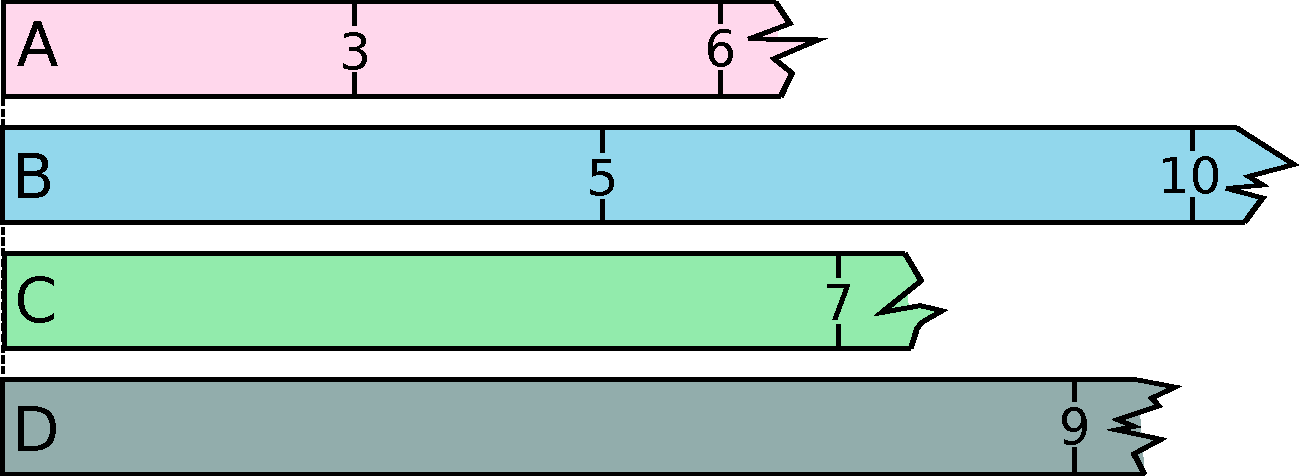
\includegraphics[scale=0.4]{media/no-04/ruban}
\end{center}
}{2}\end{exo}




\begin{exo}{
    Réponds aux questions ci-dessous.

\begin{tasks}[after-item-skip = 0.5em]
    \task Énumère les dix premiers multiples de $6$.
    \task Énumère les dix premiers multiples de $9$.
    \task Énumère les premiers multiples communs de $6$ et $9$.
    \task Tu viens de lister les premiers multiples d'un nombre. Lequel~?
    \task Quel est le plus petit multiple commun de $6$ et de $9$~?
\end{tasks}
}{2}\end{exo}

\vfill

\begin{exo}{
    Énumère les éléments de chacun des ensembles suivants.
\begin{tasks}[after-item-skip = 0.5em]
    \task L'ensemble des multiples communs de $8$ et $6$ inférieurs à $150$.
    \task L'ensemble des multiples communs de $45$ et $6$ supérieurs à $100$ et inférieurs à $500$.
\end{tasks}
}{1}\end{exo}

\vfill

\begin{exol}{NO52}{21}{2}
\end{exol}


\vfill

\begin{exo}{
    Énumère les multiples des entiers suivants, puis détermine leur plus petit multiple commun (ppmc).
\begin{tasks}(4)
    \task $3$ et $4$
    \task $2$ et $4$
    \task $6$ et $4$
    \task $3$ et $8$
    \task $6$ et $9$
    \task $5$ et $7$
    \task $11$ et $6$
    \task $3$ et $10$
\end{tasks}
}{2}\end{exo}


\vfill

\newpage

\begin{exo}{
    Calcule le ppmc des entiers suivants.

\begin{tasks}[after-item-skip = 0.5em](4)
    \task $6$ et $12$
    \task $8$ et $4$
    \task $5$ et $15$
    \task $2$ et $10$
    \task $7$ et $14$
    \task $8$ et $32$
    \task $30$ et $60$
    \task $50$ et $100$
\end{tasks}
}{2}\end{exo}


\vfill

\begin{exo}{
    Calcule le ppmc des entiers suivants.


\begin{tasks}[after-item-skip = 0.5em](4)
    \task $18$ et $24$
    \task $36$ et $60$
    \task $50$ et $70$
    \task $48$ et $36$
    \task $15$ et $20$
    \task $18$ et $20$
    \task $20$ et $30$
    \task $20$ et $25$
    \task $14$ et $35$
    \task $16$ et $6$
    \task $32$ et $5$
    \task $21$ et $12$
\end{tasks}
}{2}\end{exo}

\vfill

\begin{qmun}{Calcul du ppmc de deux nombres}{
		\begin{center}

\includegraphics[scale=1]{media/qr/neppmc1 }

\tiny{{https://edu.ge.ch/qr/neppmc1}}
		\end{center}
	}
\end{qmun}


\vfill

\begin{exo}{
    Calcule le ppmc des entiers suivants.


\begin{tasks}[after-item-skip = 0.5em](3)
    \task $5$ ; $10$ et $11$
    \task $2$ ; $4$ et $16$
    \task $10$ ; $12$  et $16$
    \task $7$ ; $14$ et $21$
    \task $3$ ; $4$ ; $5$ et $6$
    \task $2$ ; $5$ ; $8$ et $10$
\end{tasks}
}{2}\end{exo}



\vfill

\newpage

\begin{exo}{
    Les affirmations suivantes sont-elles vraies ou fausses~? Justifie ta réponse.
\begin{tasks}[after-item-skip = 0.5em]
    \task Tous les multiples de 3 sont des multiples de 6.
    \task Tous les multiples de 20 sont des multiples de 5.
    \task Tous les nombres pairs sont multiples de 4.
    %\task Plus un nombre est grand, plus il a de diviseurs.
\end{tasks}
}{2}\end{exo}


\begin{resolu}{Résolution de problèmes}{

    Anaïs s'entraîne à la course tous les 3 jours et Clara tous les 4 jours. 

    Si Anaïs et Clara sont allées à l'entraînement ensemble aujourd'hui, dans combien de temps vont-elles de nouveau courir le même jour~? 

    {\color{blue}
        Anaïs ira courir dans 3 jours, dans 6 jours, dans 9 jours, etc. 

	Cela revient à lister les multiples de 3 : 
	\[M_3=\{0~;~3~;~6~;~9~;~12~;~15~;~18~;~21~;~24~;~etc.\}\]
        Clara ira courir dans 4 jours, dans 8 jours, dans 12 jours, etc. 

	Cela revient à lister les multiples de 4 :
	\[M_4=\{0~;~4~;~8~;~12~;~16~;~20~;~24~;~28~;~etc.\}\] 
        Ainsi, Anaïs et Clara se retrouveront dans 12 jours et dans 24 jours. On remarque que cela se reproduira encore dans 36 jours, dans 48 jours, etc. Cela revient à lister les multiples communs de 3 et 4, soit les multiples de 12. 
    }
}{2}\end{resolu}


\newpage
:
\begin{exo}{
    Dans le cours de musique, Taylan frappe dans ses mains tous les 6 temps et Kathleya donne un coup de cymbales tous les 8 temps.
    \begin{tasks}[after-item-skip = 0.2em, after-skip=-0.5em, before-skip=-0.5em]
        \task À combien de temps, Taylan donnera-t-il un coup de cymbales en même temps que Kathleya frappera dans ses mains~?
        \task Au bout de combien de temps, à partir du début de la pièce, cela se répétera-t-il une autre fois~?
    \end{tasks}
}{2}\end{exo}



\begin{exo}{
    Trois bergers comptent le nombre de moutons du troupeau.

    Pour le premier berger qui a l'habitude de les compter par groupes de 6, il en reste 5. 

    Pour le deuxième berger qui a l'habitude de les compter par groupes de 8, il en reste 5.

    Pour le troisième berger qui a l'habitude de les compter par groupes de 12, il en reste 5 aussi. 

Sachant que le troupeau comporte entre 470 et 500 têtes, quel est le nombre de moutons~?

}{3}\end{exo}



\begin{exol}{NO34}{18}{1}
\end{exol}

\begin{exol}{NO35}{18}{1}
\end{exol}

\begin{exol}{NO40}{19}{1}
\end{exol}

\begin{exol}{NO41}{20}{2}
\end{exol}

\begin{exol}{NO42}{20}{1}
\end{exol}

\begin{exol}{NO43}{20}{2}
\end{exol}






\end{document}
